% This is LLNCS.DOC the documentation file of
% the LaTeX2e class from Springer-Verlag
% for Lecture Notes in Computer Science, version 2.4
\documentclass{llncs}
\usepackage{llncsdoc}

\usepackage{graphicx}
%\usepackage{balance}  % for  \balance command ON LAST PAGE  (only there!)
\usepackage{times,amsmath,epsfig,booktabs}
\usepackage[hyphens]{url}
\usepackage{algorithm}
\usepackage{algpseudocode}
%\usepackage{multirow}
\usepackage{listing}
\usepackage{amssymb}
\usepackage{pifont}
\usepackage{verbatim}
%\usepackage{comment}
\usepackage{subfig}
\usepackage{tikz}
\usepackage{listings}

\usepackage{xcolor,colortbl}

%Space saving packages
\usepackage{times}
%\usepackage[small,compact]{titlesec}
%\usepackage[small,it]{caption}



\newcommand{\model}{DRAM\_HARD}
\newcommand{\modelExplicit}{DRAM\_SOFT}
\newcommand{\modelPcmRam}{PCM\_RAM}

%\newcommand{\jhcomment}[1]{\noindent {\bf \\JH: #1 \\}}
\newcommand{\jhcomment}[1]{}

\definecolor{c1}{RGB}{239,247,245}
\definecolor{c2}{RGB}{188,189,220}
\definecolor{c3}{RGB}{117,107,177}
\newcolumntype{x}{>{\columncolor{c1}}c}
\newcolumntype{y}{>{\columncolor{c2}}c}
\newcolumntype{z}{>{\columncolor{c3}}c}
%
\begin{document}

\title{
On Improving Write Performance in PCM Databases}

% Three authors sharing the same affiliation.
\author{Vishesh Garg, Abhimanyu Singh, and Jayant R. Haritsa}
%
      \institute {Database Systems Lab, SERC/CSA\\
       Indian Institute of Science, Bangalore, INDIA\\
       \textbf{\email{\{vishesh, abhimanyu, haritsa\}@dsl.serc.iisc.ernet.in}}
       }
          
          
\maketitle
%\markboth{\LaTeXe{} Class for Lecture Notes in Computer
%Science}{\LaTeXe{} Class for Lecture Notes in Computer Science}
%\thispagestyle{empty}
%\begin{flushleft}
%\LARGE\bfseries Instructions for Authors\\
%Coding with \LaTeX\\[2cm]
%\end{flushleft}
%\rule{\textwidth}{1pt}
%\vspace{2pt}
%\begin{flushright}
%\Huge
%\begin{tabular}{@{}l}
%\LaTeXe{} Class\\
%for Lecture Notes\\
%in Computer Science\\[6pt]
%{\Large Version 2.4}
%\end{tabular}
%\end{flushright}
%\rule{\textwidth}{1pt}
%\vfill
%\begin{flushleft}
%\large\itshape
%\begin{tabular}{@{}l}
%{\Large\upshape\bfseries Springer}\\[8pt]
%Berlin\enspace Heidelberg\enspace New\kern0.1em York\\[5pt]
%Barcelona\enspace Budapest\enspace Hong\kern0.2em Kong\\[5pt]
%London\enspace Milan\enspace Paris\enspace\\[5pt]
%Santa\kern0.2em Clara\enspace Singapore\enspace Tokyo
%\end{tabular}
%\end{flushleft}
%

%
\begin{abstract} 

Phase Change Memory (PCM) is a new \emph{non-volatile} memory technology
that is comparable to traditional DRAM with regard to read latency,
and markedly superior with regard to storage density and idle power
consumption. Due to these desirable characteristics, PCM is expected
to play a significant role in the next generation of computing
systems. However, it also has limitations in the form of expensive
writes and limited write endurance. Accordingly, recent research 
has investigated how database engines may be redesigned to
suit DBMS deployments on the new technology.

\begin{comment}
In this paper, we explore the design of PCM-conscious database operators
for main memory organizations comprised of PCM augmented with a small
hardware-controlled DRAM buffer.  Specifically, we present modified
constructions of the ``workhorse'' database operators: \emph{sort},
\emph{hash join} and \emph{group-by}, that substantively improve the
write performance without compromising on execution times. We also
provide \emph{estimators} of the writes incurred by these techniques,
thereby facilitating integration with the database query optimizer.
\end{comment}

In this paper, we explore the design of PCM-conscious database operators
for main memory organizations comprised of PCM augmented with a small
hardware-controlled DRAM buffer. Specifically, we present modified
constructions of the ``workhorse'' database operators: \emph{sort},
\emph{hash join} and \emph{group-by}, which use existing but overlooked ``off-the-shelf'' algorithms for substantively improving the
write performance without compromising on execution times. We also
provide \emph{estimators} of the writes incurred by these techniques,
thereby facilitating integration with the database query optimizer.

The proposed techniques are implemented on a state-of-the-art
architectural simulator, which we extend to model PCM, and their
performance is assessed on a workload of TPC-H benchmark queries. Apart from
the number of writes and query response times, the algorithms are
also evaluated on their wear distributions. Our experimental results
suggest that the PCM-conscious operators collectively reduce the number
of writes by a factor of 2 to 3, while concurrently improving the query
response times by about 20 to 30\%.  Further, the wear distribution
is also appreciably smoother. In essence, our algorithms provide both short-term and
long-term benefits. These outcomes augur well for database engines that
wish to leverage the impending transition to PCM-based computing.

\end{abstract}


\section{Introduction}
\label{sec:intro}
%
Phase Change Memory (PCM) is a recently developed non-volatile memory
technology, constructed from chalcogenide glass material, that stores
data by switching between crystalline (\emph{binary 0}) and amorphous 
(\emph{binary 1}) states. Broadly speaking, it is expected to provide an attractive
combination of the best features of conventional disks (persistence,
capacity) and of DRAM (access speed). For instance, it is
about 2 to 4 times denser than DRAM, while providing a DRAM-comparable
read latency.  On the other hand, it consumes much less energy
than magnetic hard disks while providing substantively smaller write latency. Due to this suite of  desirable features, PCM technology is
expected to play a prominent role in the next generation of computing
systems, either augmenting or replacing current components in the memory
hierarchy~\cite{qureshi,zhou,lee}.

A limitation of PCM, however, is that there is a significant difference
between the read and write behaviours in terms of energy, latency and
bandwidth. A PCM write, for example, consumes 6 times more energy than
a read. Moreover, PCM has limited write endurance since a memory cell
becomes unusable after the number of writes to the cell exceed a threshold
determined by the underlying glass material. A summary representation
of the characteristics of PCM as compared to DRAM and HDD, is shown in
Table~\ref{tab:tab_pcm_char}.

From the table, it is evident that PCM-based applications need to be
redesigned to minimize both the number of writes and the skew in their
distribution across the memory cells.  Consequently, several database
researchers have, in recent times, focused their attention on devising
new implementations of the core database operators that are adapted to
the idiosyncrasies of the PCM environment (e.g.~\cite{chen,viglas}).

\begin{table}[!h] 

\caption{\bf Comparison of memory technologies \cite{chen}}
\label{tab:tab_pcm_char} 
\begin{small}
  \begin{tabular}{p{3cm}p{2.5cm}p{3cm}p{3cm}} 
  \toprule
    &  \textbf{DRAM} & \textbf{PCM} &  \textbf{HDD} \\
  \midrule
  \textbf{Read energy} & 0.8 J/GB & 1 J/GB  & 65 J/GB \\
  \textbf{Write energy} & 1.2 J/GB & 6 J/GB  & 65 J/GB \\
  \textbf{Idle power} & $\sim$100 mW/GB & $\sim$1 mW/GB  & $\sim$10 W/TB \\
  \textbf{Endurance} & $\infty$ & $10^6 - 10^8$  & $\infty$ \\
  \textbf{Page size} & 64B & 64B  & 512B \\
  \textbf{Page read latency}& 20-50ns & $\sim50 ns$  & $\sim 5ms$ \\
  \textbf{Page write latency} & 20-50$ns$ & $\sim 1 \mu$s  & $\sim5ms$ \\
  \textbf{Write bandwidth}  & $\sim$GB/s per die & 50-100 MB/s per die  & $\sim$200 MB/s per drive \\
  \textbf{Density} & $1\times$ & 2-4$\times$ & N/A \\
  \bottomrule 
  \end{tabular} 
\end{small} 
\end{table}

%\newpage
\subsection*{Architectural Model}
The prior database work has primarily focused on computing
architectures wherein either (a) PCM completely replaces the
DRAM memory~\cite{chen}; or (b) PCM and DRAM co-exist side-by-side
and are independently controlled by the software~\cite{viglas}. We
hereafter refer to these options as {\bf \modelPcmRam{}} and
{\bf \modelExplicit{}}, respectively.

However, a third option that is gaining favor in the architecture
community is where the PCM is augmented with a small hardware-managed
DRAM buffer~\cite{qureshi}. In this model, which we refer to as
{\bf \model{}}, the address space of the application maps to PCM and the
DRAM buffer can simply be visualized as yet another level of the existing
cache hierarchy.  For ease of comparison, these various configurations
are pictorially shown in Figure~\ref{fig:pcm_models}.

\begin{figure}[htbp]
	\includegraphics[height=50mm]{PCM_Models.png}\centering
	\caption{PCM-based Architectural Options}
	\label{fig:pcm_models}
\end{figure}
 
We, for the first time in the literature, design and evaluate algorithms
that are tuned to the \model{} model. Note that though this model was mentioned in
\cite{chen}, the design and evaluation was carried out only for \modelPcmRam{}.
There are several practical advantages of the \model{} configuration:
First, the write latency drawback of \modelPcmRam{} can be largely
concealed by the intermediate DRAM buffer~\cite{qureshi}. Second,
existing applications can be used \textit{as is} but still manage to take
advantage of both the DRAM and the PCM. This is in stark contrast to the
\modelExplicit{} model which requires incorporating additional machinery,
either in the program or in the OS, to distinguish between data mapped
to DRAM and to PCM -- for example, by having separate address space
mappings for the different memories.

\subsection*{Our Work}

\begin{comment}
In this paper, we investigate the design and evaluation of query execution
engines for the \model{} memory model.  Specifically, we propose modified
PCM-conscious implementations of the ``workhorse'' database operators:
\textit{sort}, \textit{hash join} and \textit{group-by}, that reduce
\emph{both} query writes and response times. Note that it is trivially
easy to reduce writes by \emph{sacrificing} the response times --
for instance, by replacing quicksort with selection sort, or hash join
with nested-loops join. However, our solutions reduce the writes while
concurrently \emph{improving} the timeliness of the query results.
\end{comment}

In this paper, we investigate the design and evaluation of query execution
engines for the \model{} memory model.  Specifically, we propose modified
PCM-conscious implementations of the ``workhorse'' database operators:
\textit{sort}, \textit{hash join} and \textit{group-by}, that reduce
\emph{both} query writes and response times.  Note that it is trivially
easy to reduce writes by \emph{sacrificing} the response times --
for instance, by replacing quicksort with selection sort, or hash join
with nested-loops join. However, our solutions reduce the writes while
concurrently \emph{improving} the timeliness of the query results. These implementations leverage existing "off-the-shelf" algorithms that have hitherto been overlooked for the specific application of reducing writes. The results show that we can reap significant benefits by replacing PCM oblivious operators with their PCM conscious versions. The new algorithms share most of the code with existing operator implementations indicating their ease of incorporation in existing systems.



We have implemented the modified operators on Multi2sim \cite{multi2sim},
a state-of-the-art architectural simulator, after incorporating a
major extension to support the modelling of PCM.  The performance of
the operators is evaluated on \emph{complete} TPC-H benchmark queries --
this is a noteworthy point since earlier studies of PCM databases had only
considered operator performance in isolation.  But, it is possible that
optimizing a specific operator may be detrimental to other downstream
operators that follow it in the query execution plan. For instance,
the proposal in \cite{chen} to keep nodes unsorted in B$^+$ indexes,
while saving on writes, can be detrimental to the running times of
subsequent operators, e.g. join filters, that leverage index ordering.

The experimental results suggest that, as compared to the original
PCM-oblivious operators, our new implementations collectively offer
substantive benefits with regard to PCM writes -- the number is typically
brought down \emph{by a factor of two to three}.  Concurrently, the query
response times are also brought down by about \emph{20 to 30 percent}.
As a sample case in point, for TPC-H Query 19, savings of 64\% in PCM
writes are achieved with a concomitant 32\% reduction in CPU cycles.

A unique feature of our analysis is that we also evaluate the writes with
regard to their \emph{distribution} over the memory cells. This is because
a skewed distribution adversely impacts the endurance of cells with high
write rates, raising the frequency at which wear-leveling mechanisms
have to be put into play by the system. We observe that our algorithms don't introduce any new skew while achieving the reduction in writes and cycles.

Finally, we provide simple approximate mathematical \emph{estimators} for the
number of writes incurred by the new operators and validate them in our
experiments. These estimators are then incorporated in the query optimizer's
cost model to come up up with the most suitable plan in this new paradigm.

In a nutshell, the new PCM-conscious operators proposed in this paper
provide both \emph{short-term and long-term performance benefits}.
Overall, these outcomes augur well for the impending migration of database
engines to PCM-based computing platforms.

\subsection*{Organization}
The remainder of this paper is organized as follows: We define the
problem framework in Section~\ref{assumptions}. The design of the new
PCM-conscious database operators, and their theoretical analysis,
are presented in Sections~\ref{sort}, \ref{hj} and \ref{gby}.
Our experimental framework and the simulation results are reported in
Sections~\ref{sec:exp} and \ref{sec:results}, respectively. This is followed by a
discussion on optimizer integration in Section~\ref{discussion}. The
related literature is reviewed in Section~\ref{relWork}. Finally,
Section~\ref{conclusion} summarizes our conclusions and outlines future
research avenues.


\section{Problem Framework}
\label{assumptions}
In this section, we overview the problem framework, the assumptions made
in our analysis, and the notations used in the sequel.

As mentioned in the Introduction, we model the \model{} memory
organization (Figure~\ref{fig:pcm_models} (c)). The DRAM buffer is of
size $D$ and is organized in a \emph{K-way set-associative} manner, like the higher level cache memories. Moreover, its operation is also identical to that of an \emph{inclusive} cache in the memory hierarchy; fetching a new DRAM line (256B in our experimental setup) from PCM each time there is a DRAM miss. The last level cache in turn fetches its data from the DRAM buffer.

A \textit{data-comparison write (DCW)} scheme \cite{write} is used for
the writing of PCM memory blocks during eviction from DRAM -- in this
scheme, the memory controller compares the existing PCM block to the newly
evicted DRAM block, and selectively writes back only the modified words.
Further, \textit{N-Chance}~\cite{nchance} is used as the DRAM eviction
policy -- here, the first clean way in the $N$ least recently used ways
(assuming $N$ is less than $K$, the DRAM cache associativity) in a set
is chosen as the eviction victim. Only when all the $N$ ways are dirty,
the LRU entry is evicted. We choose this scheme due to its preference
for evicting non-dirty entries over dirty candidates, thereby saving
on writes.

As described above, the simulator implements a realistic DRAM
buffer. However, in our write analyses and estimators, we assume for
tractability that there are no conflict misses in the DRAM. Thus, for
any operations dealing with data whose size is within the DRAM capacity,
our analysis assumes no evictions and consequently no writes.

With regard to the operators, we use $R$ to denote the input relation
for the \textit{sort} and \textit{group-by} unary operators.  Whereas,
for the binary \textit{hash join} operator, $R$ is used to denote the
smaller relation, on which the hash table is constructed, while $S$
denotes the probing relation. 

We assume that all the input relations are completely PCM-resident.
Further, for simplicity of presentation, we assume that the sort,
hash-join and group-by expressions are on single relational attributes --
the extension to multiple attributes is straightforward.

A summary of the main notation used in the analysis of the following
sections is provided in Table~\ref{tab:notations}.

\begin{table}[!h]
\centering
\caption{Notations Used in Operator Analysis}
\label{tab:notations}
\begin{small}
\begin{tabular}{p{2cm}p{9cm}}
\toprule  
\textbf{Term} & \textbf{Description}\\ 
\midrule
\textbf{$D$} & DRAM size\\
\textbf{$K$} & DRAM Associativity\\
\textbf{$P$} & Pointer size\\
\textbf{$N_R, N_S$} & Row cardinality of relations R and S, respectively\\
\textbf{$L_R, L_S$} & Tuple size of relations R and S, respectively\\
\textbf{$size_{entry}$} & Size of each hash table entry\\
\textbf{$J,G$} & Output tuple cardinalities of join and group-by operators, respectively\\
\textbf{$size_{j},size_{g}$} & Output tuple sizes of join and group-by operators, respectively\\
\bottomrule
\end{tabular}
\end{small}
\end{table}


\section{The Sort Operator}
\label{sort}

Sorting is among the most commonly used operations in database systems,
forming the core of operators such as \emph{merge-join}, \emph{order-by} and
some flavors of \emph{group-by}.  The process of sorting is quite
write-intensive since the commonly used in-memory sorting algorithms,
such as \textit{quicksort}, involve considerable data movement. In the
single pivot quicksort algorithm with $n$ elements, the average number
of swaps is of the order of $0.3nln(n)$~\cite{swaps}.  There are other
algorithms such as \emph{selection sort} which involve much less data
movement, but they incur \emph{quadratic} time complexity in the number
of elements to be sorted, and are therefore unsuitable for large datasets. Algorithms like \emph {merge sort}, on the other hand, require additional space for the merge step which is undesirable given the limited space availability in PCM.

The quicksort algorithm divides the input array into two partitions in each partitioning step. If the initial array is much larger than the DRAM size, it would
entail evictions from the DRAM during the swapping process of
partitioning. These evictions might lead to PCM writes if the evicted
DRAM lines are \textit{dirty}, which is likely since elements are being
swapped. If the resulting partition sizes continue to be larger than
DRAM, partitioning them in turn will again cause DRAM evictions and
consequent writes. Clearly, this trend of writes will continue in the
recursion tree until the partition sizes become small enough to fit within
DRAM. Thereafter, there would be no further evictions during swapping
and the entire subsequent sorting process would finish within the DRAM.

From the above discussion, it is clear that it would be desirable for a sorting algorithm to be in-place, converge fast to partition sizes within DRAM size with less amount of swaps, and yet be reasonably fast. We pick an alternate algorithm - flashsort \cite{flashsort} - which has these properties. Specifically, flashsort can potentially form DRAM sized partitions in a \emph{single} partitioning step with at most $N_R$ swaps. The sorting is done in-place with a time complexity of $O(N_Rlog_2N_R)$ with constant extra space\footnote{The time complexity can be brought down to $O(N_R)$ with $O(N_R)$ extra space}. The flashsort algorithm proceeds in three phrases: \emph{Classification Phase}, \emph{Permutation Phase} and \emph{Short-range Ordering Phase}. The classification phase divides the input data into $p$ partitions where $p$ is given as input. Given an element with value $v$, $Partition(v) = 1 + \lfloor \frac{(p-1)(v- v_{min})}{v_{max}-v_{min}} \rfloor$; $v_{min}$ and $v_{max}$ being the smallest and the largest values in the array, respectively. It then counts the number of elements in each such partition to get the boundary information. The permutation phase moves the elements to their respective partitions. The individual partitions are then finally sorted in the Short-range Ordering Phase to get the overall sorted array.

We choose the number of partitions $p$ to be $\lceil c \times \frac{N_R L_R}{D} \rceil$, where $c \geq 1$ is a design
parameter. This is because if we were to go with $p$ to be exactly $\frac{N_R L_R}{D}$, some partitions might turn out to be larger than the DRAM size if the data is not uniformly distributed. In our experience, setting $c = 2$ worked well in practice.

%\begin{algorithm}
\small
\caption{Read Phase}
\label{alg:read_phase}
\textbf{array[]} is the array of input tuples\\
\textbf{c} is a design parameter $\geq 1$\\
\begin{algorithmic}[1]
\State p = $\lceil c\times \frac{N_R L_R}{D} \rceil$
\State randIndex[] = generate $p-1$ random indexes
\State pivot[] = array[randIndex];
\State sort(pivot[])
\State size[] = {0...0}   
\Comment{size of sub-arrays}
\For {i=$1$ to $N_R$}
\State partition = getPartition(array[i]) 
\State size[partition]++ 
\EndFor
\Comment {Time complexity=$N_R\times log_2p$ }
\State cumulative = 0
\For {i=$1$ to $p$}
\State cumulative = cumulative + size[i]
\State partitionStart[i+1] = cumulative
\EndFor
\Comment {Time complexity=$p$ }
\State return partitionStart[]
\end{algorithmic}

\end{algorithm}


For partitions that turn
out to be within the DRAM size, the Short-range Ordering phase is completed using
quicksort. On the other hand, if some larger-sized
partitions still remain, we recursively apply the flashsort
algorithm to sort them until all the resulting partitions fit within DRAM and finish sorting with lesser evictions.

\textbf{PCM write analysis}: Though the partition boundary counters
are continuously updated during the Classification phase, they are expected to
incur very few PCM writes. This is because since all those updates are
in quick succession, the counters are unlikely to be evicted from DRAM
\emph{during} the update process. During the
Permutation phase, there will be no more than $N_R L_R$ writes since each tuple is written
at most once while placing it within its partition boundaries. If each
partition is within the DRAM size, the Short-range Ordering phase (for each partition)
will finish within DRAM and there will be another $N_R L_R$ writes upon
eventual eviction of sorted partitions to PCM. 

Thus, in the average case of uniform data distribution, the writes incurred by this algorithm is estimated by
\begin{equation}
\label{eq:mpivot}
  W_{sort} = 2N_RL_R
\end{equation}

\section{The Hash Join Operator}
\label{hj}
Hash join is perhaps the most commonly used of all join algorithms in
database systems. Here, a hash table is built on the smaller relation,
and tuples from the larger relation are used to probe for matching values
in the join column. Since we assume the table is completely PCM-resident, the join here \emph{does not} require any initial partitioning stage. Instead, we directly proceed to the join phase. Thus, during the progress of hash join,
writes will be incurred during the building of the hash table, and also
during the writing of the join results.

In the following subsections, we first discuss the conventional hash table
construction, followed by our PCM-conscious modifications. We assume $size_{entry}$
to be the hash table entry size for each tuple of the build relation.
Further, if the result of the join is $J$ join tuples, each of size
$size_{j}$, then the total \emph{output} writes, which is common to all
algorithms, would be $J \times size_{j}$. We ignore the writes incurred while initializing each hash table bucket since they are negligible in comparison to inserting the actual entries.

\subsection{Conventional hash table}
Each entry in the hash table consists of a pointer to the corresponding
build tuple and the hash value for the join column. Due to the
absence of prior knowledge about the distribution of join column values
for the build relation, the hash table is expanded dynamically according
to the input. Typically, for each insertion in a bucket, a new space is
allocated and is connected to existing entries using a pointer. Thus,
such an approach incurs an additional pointer write each time a new
entry is inserted.

\textbf{PCM write analysis}: 
For each new entry, there would typically be a pointer write (of size $P$ bytes),
apart from the $size_{entry}$ bytes for the entry itself.  Thus the total writes 
for conventional hash table is given by
\begin{equation}\label{eq:ht_conv}
  W_{ht\_conv} = N_R \times (size_{entry} + P) + J \times size_{j}
\end{equation}

\subsection{PCM-conscious hash table}
We now move on to discussing hash table construction optimizations that
can reduce the number of PCM writes.

\subsubsection{Bitmapped page based allocation}
Our first improvement is to allocate space to hash buckets in units of
fixed size called \textit{pages}. A page contains a set of contiguous
entries, the maximum count of entries being fixed depending on the size
of the page and the size of the entry. When a page overflows a new page
is allocated and linked to the overflowing page via a pointer.  Thus,
unlike the conventional hash table wherein each \emph{pair} of entries
are connected using pointers, the interconnecting pointer here is only
at page granularity. Note that although using open-addressing is another method of avoiding pointers, probing for a join attribute value would have to search through the entire table each time. This is because the inner table might contain multiple tuples with the same join attribute value and thus the probe cannot terminate without looking at the entire hash table.   

A control bitmap is used to indicate whether each entry in a page is vacant
or occupied, a necessary information during both insertion and search in the
hash table. Each time a bucket runs out of space, a new page is allocated
to the bucket. Though such an approach  may lead to space wastage when
some of the pages are not fully occupied, we save on the numerous pointer
writes that are incurred when space is allocated on a per-entry basis.

\textbf{PCM write analysis}: Assuming there are $E_{page}$ entries per page, there would now be one pointer per $E_{page}$ entries. Additionally, for each insertion, a bit write would be incurred due to the bitmap update. In such a case, the writes would be 
$$W_{ht\_bitmapped} = N_R \times (size_{entry} +  \frac{P}{E_{page}} + \frac{1}{8} ) + J \times size_{j}$$\\
Since in practice both  $\dfrac{P}{E_{page}}$ and $\dfrac{1}{8}$ are small as compared to $size_{entry}$, 
\begin{equation}\label{eq:ht_bmp}
 W_{ht\_bitmapped} \approx N_R \times size_{entry} + J \times size_{j} 
\end{equation} 


\subsubsection{Reducing hash value length}
We can reduce the writes incurred due to storing of the hash values in
the hash table by restricting the length to just a single byte. In this
manner, we trade-off precision for fewer writes. If the hash function
distributes the values in each bucket in a perfectly uniform manner, it
would be able to distinguish between $2^8 = 256$ join column values in a
bucket. This would be sufficient if the number of distinct values mapping
to each bucket turn out to be less than this value. Otherwise, we would
have to incur the penalty (in terms of latency) of reading the actual join
column values from PCM due to the possibility of false positives.

\textbf{PCM write analysis}: Let us assume the original hash value
was four bytes long. Using a single byte hash value instead, combined
with a bitmapped page based hash table, leads to the total writes of
$W_{ht\_pcm}$ being given by
\begin{equation}\label{eq:ht_pcm}
W_{ht\_pcm} = N_R \times (size_{entry} - 3)+ J \times size_{j}
\end{equation}
	



\section{The Group-By Operator}%
\label{gby}
We now turn our attention to the group-by operator which typically
forms the basis for aggregate function computations in SQL queries.
Common methods for implementing group-by include \textit{sorting} and
\textit{hashing} -- the specific choice of method depends both on the
constraints associated with the operator expression itself as well as
on the operators following later in the plan tree.

In the following subsections, we begin by considering the hash-based
group-by operator and present our modifications of this technique for
the PCM environment. Subsequently, we move on to a similar discussion
for sort-based group-by implementations.

Note that if we assume the result of the group-by to be $G$ tuples,
each of $size_g$, then the total \emph{output} writes, which is common
to all algorithms, would be $G \times size_g$.

\subsection{Hash Based Grouping}

\subsubsection{Conventional group-by}
A hash table entry for group-by, as compared to the corresponding
entry in hash join, has an additional field containing the aggregate
value. For each new tuple in the input array, a bucket index is
obtained after hashing the value of the column present in the group-by
expression. Subsequently, a search is made in the bucket indicated by
the index. If a tuple matching the group-by column value is found, the
aggregate field value is updated; else, a new entry is created in the
bucket. Thus, unlike hash join, where each build tuple had its individual
entry, here the grouped tuples share a common entry with an aggregate
field that is constantly updated over the course of the algorithm.

\textbf{PCM write analysis}: The number of separate entries in the
hash table is $G$, incurring $G \times size_{entry}$ writes. If
$size_{agg\_field}$ represents the size of the aggregate field
during grouping, the writes due to each update of the aggregate would be $N_R \times
size_{agg\_field}$. This
would give the total number of writes as:
\begin{equation}
\label{eq:gby_conv_ht}
\begin{split}
W_{gb\_conv\_ht} = G \times (size_{entry} + P) + \\
N_R \times size_{agg\_field} + G \times size_g
\end{split}
\end{equation}

\jhcomment{Again worst case! Discuss!}

\subsubsection{PCM-conscious group-by}
Since the hash table construction for group-by is identical to that
of the hash-join operator, the PCM-related modifications described
in Section~\ref{hj} can be applied here as well. That is, we employ
a page-based hash table organization, and a reduced hash value size,
to reduce the writes to PCM.

\textbf{PCM write analysis}: From the above discussion, it is easy to see
that the total writes incurred for the PCM-conscious is given by
\begin{equation}
\begin{split}
W_{gb\_opt\_ht} = G \times (size_{entry} - 3) + \\
N_R \times size_{agg\_field} + G \times size_g
\end{split}
\end{equation}

\subsection{Sort Based Grouping}

Sorting may be used for group-by when a fully ordered operator such
as \textit{order by} or \textit{merge join} appears downstream in the plan
tree. Another use case is for queries with a \textit{distinct} clause
in the aggregate expression, in order to identify the duplicates that have
to be discarded from the aggregate.  

\begin{comment}
A sample case in point is the following SQL query: \\
\begin{small}
\hspace*{0.5in}	{\sf select o.customer, count(distinct(o.orderID))} \\
\hspace*{0.5in}	{\sf from orders as o}  \\
\hspace*{0.5in}	{\sf group by o.customer}
\end{small}
\end{comment}


\begin{comment}
Sorting thus is a commonly used technique for grouping but it incurs
its corresponding large number of writes.
In such a case, we can now no longer simply update the aggregate values in the hash table for group-by since the existence of duplicates needs to be checked in parallel. To get past this limitation, query optimisers usually choose to use sorting for aggregation. Since the group of tuples forming each aggregate now reside contiguously in the sorted list, duplicates can be identified easily and eliminated, while performing the aggregation.
\end{comment}


\subsubsection{Conventional group-by}
\textbf{PCM write analysis}: For sort-based grouping, the writes would
be akin to those incurred for sorting. Thus, following the same analysis
as in Equation \ref{eq:sort_conv}, the total writes would be:
\begin{equation}
\label{eq:gby_conv_sort}
W_{gb\_conv\_sort} = N_RL_R (0.5 \lceil log_2(\frac{N_R L_R}{D}) \rceil + 1) + G \times size_g
\end{equation}	


\subsubsection{PCM-conscious ordered group-by}
\label{subsec:gb_ptr_mpivot} 
Sorting based group-by differs in a key aspect from conventional sorting
in that that the sorted tuples do not have to be written out. Instead, it
is the aggregated tuples that are finally passed on to the next operator
in the plan tree. Hence, we can modify the multi-pivot quicksort of
Section~\ref{subsec:sort_mpivot} to use \emph{pointers} in both the
\textit{Swap} and \textit{Sort} phases, subsequently leveraging these
pointers to perform aggregation on the sorted tuples.

\textbf{PCM write analysis}: The full tuple writes of $2 N_R L_R$
which were incurred in the multi-pivot quicksort scheme, are
now replaced by $2N_R \times P$ since pointers are used during
both the partitioning and sorting phases. Thus, the total writes for this
algorithm would be:
\begin{equation}
\label{eq:gby_ptr_mpivot}
W_{gb\_ptr\_mpivot} = 2N_R \times P + G \times size_g
\end{equation}

\subsubsection{PCM-conscious distinct group-by}
\begin{algorithm}[h!]
\caption{PCM-conscious distinct grouping}
\label{alg:hash_based_pcm_partition}
\begin{algorithmic}[1]
\State $ p = c\times \frac{N_R L_R}{D}$;
\State $ size[] = {0..0}$;   
\Comment{size of sub-arrays}\\
\textbf{Read Phase}
\For {i=$1$ to $N_R$}
\State partition = hash(array[i]) 
\State size[partition]++ 
\EndFor
\Comment {Time complexity=$N_R$ }
\State cumulative = 0
\For {i=$1$ to $p$}
\State cumulative = cumulative + size[i]
\State partitionStart[i+1] = cumulative
\EndFor
\Comment {Time complexity=$p$}\\
\textbf{Swap Phase}
\State Similar to multi-pivot quicksort swap phase presented in Algorithm~\ref{alg:swap_phase} with tuple swapping replaced by pointer-to-tuple swapping, and binary search within pivots replaced by hashing.
\Comment {Time complexity=$N_R$ }
\State return partitionStart[];
\end{algorithmic}
\end{algorithm} 
For group-by with the \textit{distinct} clause, the \emph{entire} array
need not be sorted, the only requirement being that all the members of a
group be collocated. Therefore, a pivot-based division of the array is no
longer necessary. Instead, hashing can be used to divide the input tuples
into DRAM-sized partitions. These partitions are then internally sorted by means
of pointers, just as in the pointer-based multi-pivot algorithm described above. 

Though this methodology does not reduce the writes as compared to 
pivot-based partitioning, it helps bring down the time complexity of
moving the tuples to the right partitions. This is because we do not have
to perform a binary search within the sorted list of pivots to identify
the range to which a column value belongs. Instead, a direct
hash of the column value can determine the correct partition for
the tuple. The modified partitioning pseudo-code is shown below
in Algorithm~\ref{alg:hash_based_pcm_partition}.



As we can see, hash-based partitioning brings down the time complexity
of both the read phase and the swap phase to $N_R$ from $N_R \times
log_2p$ while retaining the write efficiency of pointer-based multi-pivot
quicksort grouping.


\textbf{PCM write analysis}: The expected writes are the same as that
of PCM-conscious ordered grouping (Equation~\ref{eq:gby_ptr_mpivot}), i.e. 
\begin{equation}
\label{eq:gby_ptr_hash}
W_{gb\_ptr\_hash} = 2N_R \times P + G \times size_g
\end{equation}



%\subsection*{Unitary increment based Group-by}
%There can be cases where the Hash Table size is much larger than the DRAM and the group-by aggregate field involves a counter that undergoes unit increments. A sample case in point is the \textit{Count} aggregate function. A simple binary counter can lead to an arbitrary number of writes during intermediate evictions. For e.g., consider a counter having a decimal value of $2$ represented by a 3-bit binary value of $010$. An increment would change it to $011$ incurring a 1 bit write. A subsequent increment however would change it to $100$ leading to 3 bit writes. For such scenarios, we propose counters based on \textit{Gray Codes} \cite{gray_code}. The Gray Code representation between two contiguous count value differs by a single bit. For the previous example, the next gray code value after $011$ will be $111$. Thus, in the case where there is a high probability of each successive count value getting evicted, the writes per eviction would be close to a few bits.


\section{Simulation Testbed}
\label{sec:exp}

This section details our experimental settings in terms of the hardware
parameters, the database and query workload, and the performance metrics
on which we evaluated the PCM-conscious operator implementations.



\subsection{Architectural Platform}
Since PCM memory is as yet not commercially available, we
have taken recourse to a simulated hardware environment to
evaluate the impact of the PCM-conscious operators.  For this
purpose, we chose Multi2sim~\cite{multi2sim}, an open-source
application-only\footnote{Simulates only the application layer without
the OS stack.} simulator that can model a multithreaded, multicore,
superscalar x86 CPU and an AMD Evergreen GPU. It has support for both
functional simulation and cycle-accurate detailed architecture simulation.

We evaluated the PCM-conscious algorithms on Multi2sim in cycle-accurate simulation
mode. Since it does not have native support for PCM, we made a major
extension to its existing memory module to model PCM with a hardware-controlled DRAM buffer as main memory. Furthermore, we added separate data tracking functionality
for the DRAM and PCM-resident data, to implement the DCW scheme of DRAM line writeback to PCM discussed in Section \ref{sec:framework}. Likewise, we made several other enhancements to Multi2sim for PCM modelling, and these are exhaustively covered in \cite{techreport}.

\begin{center}
\begin{table}[t]
\begin{small}
\caption{Experimental Setup}
\label{table:setup}
\begin{tabular}{p{3cm}p{9cm}}
\toprule
Simulator & Multi2sim-4.2 with added support for PCM\\ \hline

L1D cache (private) & 32KB, 64B line, 4-way set-associative, 4 cycle latency, write-back, LRU\\ \hline
L1I cache (private) & 32KB, 64B line, 4-way set-associative, 4 cycle latency, write-back, LRU\\ \hline   
L2 cache (private) & 256KB, 64B line, 4-way set-associative, 11 cycle latency, write-back, LRU\\ \hline

DRAM buffer (private) & 4MB, 256B line, 8-way set-associative, 200 cycle latency, write-back, N-Chance (N = 4)\\ \hline

Main Memory & 2GB PCM, 4KB page, 1024 cycle read latency (per 256B line), 64 cycle write latency (per 4B modified word)\\ \bottomrule
\end{tabular}
\end{small}
\end{table}
\end{center}

\vspace{-0.4in}
The specific configurations used in the memory hierarchy \emph{(L1 Data,
L1 Instruction, L2, DRAM Buffer, PCM)} evaluated in our experiments are
enumerated in Table~\ref{table:setup}.  These values are scaled down
versions, wrt number of lines, of the hardware simulation parameters used
in \cite{wear} -- the reason for the scaling-down is to ensure that the
simulator running times are not impractically long. However, we have been
careful to ensure that the \emph{ratios} between the sizes of adjacent
levels in the hierarchy are maintained as per the original configurations
in \cite{wear}.  

%\vspace*{0.05in}

\subsection{Database and Queries}
%We used TPC-H (version 2.16.0) 1GB PCM-resident database for our experiments.
For the data, we used the default 1GB database generated by the TPC-H
benchmark.  This size is certainly small compared to the database sizes
typically encountered in modern applications -- however, we again chose
this reduced value to ensure viable simulation running times. Nevertheless, this database is significantly larger than the simulated DRAM (4MB), a faithful representation of most real-world scenarios.

For simulating our suite of database operators -- \textit{sort},
\textit{hash join} and \textit{group by} -- we created a separate library
consisting of the native PostgreSQL implementation of these operators. To
this library, we added the PCM-conscious versions described in the
previous sections.

While we experimented with several of the TPC-H queries, results for
three queries: Query 13 (Q13), Query 16 (Q16) and Query 19 (Q19), that
cover a diverse spectrum of the experimental space, are presented here.
For each of the queries, we first identified the query execution plan
recommended by the PostgreSQL query optimizer with the native operators,
and then forcibly used the same execution plan for their PCM-conscious
replacements as well. This was done in order to maintain fairness in the
comparison of the PCM-oblivious and PCM-conscious algorithms, though it
is possible that a better plan is available -- we return to this issue 
later in Section~\ref{discussion}. 

The execution plans associated with the three queries are shown in Figure~\ref{fig:plan_trees}. 
 


\begin{figure*}[t]
\centering
\subfloat[Q13]{
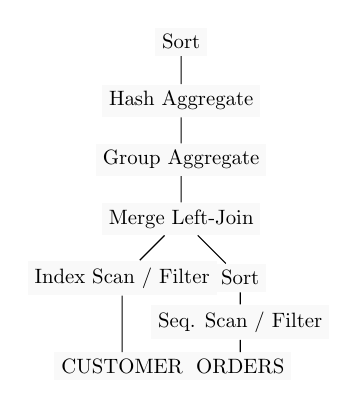
\begin{tikzpicture}[scale=.75, transform shape]

\tikzstyle{every node} = [rectangle, fill=gray!5]

\node (d) at (0,3) {Index Scan / Filter};
\node (c) at (0,1.5) {CUSTOMER};

\node (s) at (2,3) {Sort};
\node (p) at (2,2.25) {Seq. Scan / Filter};
\node (a) at (2,1.5) {ORDERS};

\node (e) at (1,4) {Merge Left-Join};
\node (f) at (1,5)  {Group Aggregate};
\node (g) at (1,6)  {Hash Aggregate};
\node (h) at (1,7)  {Sort};


\draw[-] (c) -- (d);
\draw[-] (a) -- (p);
\draw[-] (d) -- (e);
\draw[-] (p) -- (s);
\draw[-] (s) -- (e);
\draw[-] (e) -- (f);

\draw[-] (f) -- (g);
\draw[-] (g) -- (h);

\end{tikzpicture}
}
\subfloat[Q16]{
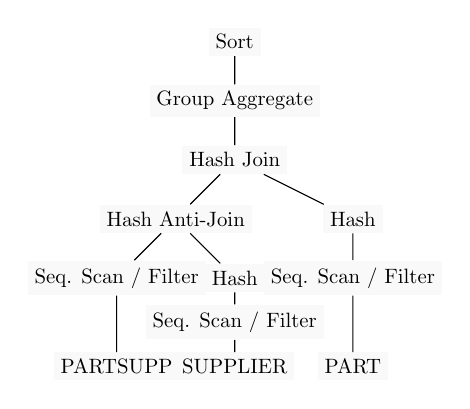
\begin{tikzpicture}[scale=.75, transform shape]

\tikzstyle{every node} = [rectangle, fill=gray!5]

\node (d) at (0,3) {Seq. Scan / Filter};
\node (c) at (0,1.5) {PARTSUPP};

\node (s) at (2,3) {Hash};
\node (p) at (2,2.25) {Seq. Scan / Filter};
\node (a) at (2,1.5) {SUPPLIER};

\node (e) at (1,4) {Hash Anti-Join};

\node (n) at (4, 4) {Hash};
\node (b) at (4,3) {Seq. Scan / Filter};
\node (x) at (4,1.5) {PART};

\node (f) at (2,5)  {Hash Join};
\node (g) at (2,6)  {Group Aggregate};
\node (h) at (2,7)  {Sort};


\draw[-] (c) -- (d);
\draw[-] (a) -- (p);
\draw[-] (d) -- (e);
\draw[-] (p) -- (s);
\draw[-] (s) -- (e);
\draw[-] (e) -- (f);

\draw[-] (x) -- (b);
\draw[-] (b) -- (n);
\draw[-] (n) -- (f);

\draw[-] (f) -- (g);
\draw[-] (g) -- (h);

\end{tikzpicture}

}
\subfloat[Q19]{


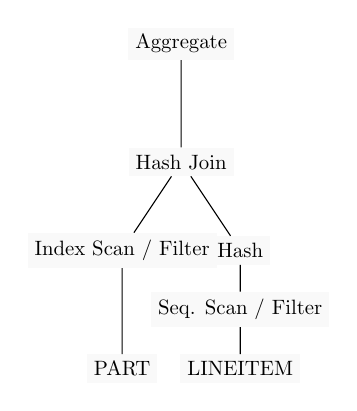
\begin{tikzpicture}[scale=.75, transform shape]

\tikzstyle{every node} = [rectangle, fill=gray!5]

\node (d) at (0,3.5) {Index Scan / Filter};
\node (c) at (0,1.5) {PART};

\node (s) at (2,3.5) {Hash};
\node (p) at (2,2.5) {Seq. Scan / Filter};
\node (a) at (2,1.5) {LINEITEM};

\node (e) at (1,5) {Hash Join};
\node (f) at (1,7)  {Aggregate};


\draw[-] (c) -- (d);
\draw[-] (a) -- (p);
\draw[-] (d) -- (e);
\draw[-] (p) -- (s);
\draw[-] (s) -- (e);
\draw[-] (e) -- (f);
\end{tikzpicture}
}

\caption{ Query execution plan trees}

\label{fig:plan_trees}

\end{figure*}




\subsection{Performance Metrics}
We measured the following performance metrics for each of the queries:
\begin{description}


\item [PCM Writes:] The total number of word (4B) updates that are applied to the PCM memory during
the query execution.
\item [CPU Cycles:] The total number of CPU cycles required to execute the query.
\item [Wear Distribution:] The frequency of writes measured on a per-256B-block basis.

\end{description}

\section{Experimental Results}
\label{sec:results}
Based on the above framework, we conducted a wide variety of experiments
and present a representative set of results here.  We begin by profiling the PCM Writes and CPU Cycles behavior of
the native and PCM-conscious executions for Q13, Q16 and Q19 --
these results are shown in Figure~\ref{fig:overall_results}.  In each of these figures, we provide both the total and
the break-ups on a per operator basis, with \emph{GB} and \emph{HJ} lables denoting Group-By and Hash Join operators, respectively.

\begin{figure*}[!h]

\centering

\subfloat[Impact of sort on overall performance - Q13]{
  \includegraphics[height=29mm]{overall_q13.png}
  
}
\hspace{0mm}
\subfloat[Impact of group-by on overall performance - Q16]{
  \includegraphics[height=29mm]{overall_q16.png}
}
\hspace{0mm}
\subfloat[Impact of hash join on overall performance - Q19]{
  \includegraphics[height=29mm]{overall_q19.png}
}
\caption{Overall performance of queries}
\label{fig:overall_results}
\end{figure*}


Focusing our attention first on Q13 in
Figure~\ref{fig:overall_results}(a), we find that the bulk of the
overall Writes and Cycles are consumed by the Sort operator. Comparing
the performance of the Native (blue bar) and PCM-conscious (green bar)
implementations, we observe a very significant savings (53\%) on Writes,
and an appreciable decrease (20\%) on Cycles.

Turning our attention to Q16 in Figure~\ref{fig:overall_results}(b),
we find that here it is the group-by operator that primarily influences
the overall Writes performance, whereas the hash-join determines the
Cycles behavior. Again, there are substantial savings in both Writes
(40\%) and  Cycles (30\%) delivered by the PCM-conscious approach.

Finally, moving on to Q19 in Figure~\ref{fig:overall_results}(c),
where hash-join is essentially the only operator, the
savings are around $64\%$ with regard to Writes and $32\%$ in Cycles.

\subsection{Operator-wise Analysis}
We now analyse the savings due to each operator independently and show
their correspondence to the analysis in Sections~\ref{sort}--\ref{gby} .

\paragraph{Sort.}
For Q13, as already mentioned, we observed savings of $53\%$ in writes and
$20\%$ in cycles.  In the case of Q16, the data at the sorting stage was
found to be much less than the DRAM size. Hence, both the native and
PCM-conscious executions used the standard sort routine, and as a result,
the cycles and writes for both implementations match exactly.

\paragraph{Hash Join.}
Each entry in the hash table consisted of a pointer to the build tuple
and a hash value field. New memory allocation to each bucket was done
in units of pages, with each page holding up to 64 entries. A search for
the matching join column began with the first tuple in the corresponding
bucket and went on till the last tuple in that bucket, simultaneously
writing out the join tuples for successful matches.  For Q16, we
observed a $12\%$ improvement in Writes and $31\%$ in Cycles due to the
PCM-conscious hash join, as shown in Figure~\ref{fig:overall_results}(b). The high savings in Cycles was the result of the caching effect due to page-wise allocation.
These improvements were even higher with Q19  -- 65\% Writes and 32\%
Cycles in Figure~\ref{fig:overall_results}(c) -- the source of the
enhancement was the 3 bytes of writes saved due to single-byte hash
values\footnote{The hash values of all entries within a bucket are placed contiguously.}, in addition to the page-based aggregation of hash table entries.


\paragraph{Group-By.}
In Q16, the aggregate operator in the group-by has an associated
\textit{distinct} clause.  Thus, our group-by algorithm utilized
hash-based in-place partitioning followed by sorting to carry out the
aggregation. Both the partitioning and sorting were carried out through
pointers, thereby reducing the writes significantly. Consequently,
we obtain savings of $74\%$ in Writes and $20\%$ in Cycles, as shown
in Figure~\ref{fig:overall_results}(b).  When we consider Q13, however,
the hash table consisted of very few entries. The less number of entries
led to the overhead of the page metadata construction overshadowing the
savings obtained in other aspects. Specifically, only marginal improvements
of about 4\% and 1\% were obtained for Writes and Cycles, as shown in
Figure~\ref{fig:overall_results}(a).

\begin{figure*}[t]
\centering

\subfloat[Q13]{
  \includegraphics[width=4cm]{wear_q13.png}
}
\subfloat[Q16]{
  \includegraphics[width=4cm]{wear_q16.png}
}
\subfloat[Q19]{
  \includegraphics[width=4cm]{wear_q19.png}
}
\caption{Queries wear distribution }
\label{fig:wear_dist}
\end{figure*}



\subsection{Lifetime Analysis}

The above experiments have shown that PCM-conscious operators
can certainly provide substantive improvements in both Writes and
Cycles. However, the question still remains as to whether these
improvements have been purchased at the expense of \emph{longevity} of
the memory. That is, are the writes skewed towards particular memory
locations?  To answer this, we show in Figure~\ref{fig:wear_dist}, the
maximum number of writes  across all memory blocks (as mentioned earlier,
we track writes at the block-level (256 bytes) in our modified simulator),
for the three TPC-H queries. The x-axis displays the block numbers in
decreasing order of writes.

We observe here that the maximum number of writes is considerably more for the
native systems as compared to the PCM-conscious processing. This
conclusively demonstrates that the improvement is with regard to
\emph{both} average-case and worst-case behavior.

\subsection{Validating Write Estimators}
\label{sec:validation}

We now move on to validating the estimators
(presented in Sections~\ref{sort} through \ref{gby})  for the number of
writes incurred by the various database operators.

\subsubsection{Sort}
The size of the $orders$ table is approximately $214 \times 10^6$ bytes. 
The flashsort algorithm incurred writes of $110.6 \times 10^6$ words $= 441.8 \times 10^6 $
bytes. Replacing the values for $N_R L_R$ with the table size in Equation \ref{eq:sort},
we get the writes as 
\begin{small}
$$W_{sort}(bytes) = 2 \times 214 \times
10^6  = 428 \times 10^6 $$ 
\end{small}
Thus the estimate is close to the observed writes.



\subsubsection{Hash Join}
For the hash join in Q19, the values of $N_R$, $size_{entry}$, $J$,
$size_{j}$ are $2 \times 10^5$, $5$ bytes, $120$ and $8$ bytes, respectively. 
Substituting the parameter values in Equation \ref{eq:hj}, the writes are given by:  
\begin{small}
$$W_{hj}(bytes) = 2 \times 10^5 \times 5 + 120 \times 8 \approx 10^6$$
\end{small}
which is close to the actual writes of $0.32 \times 10^6$ words $=
1.28 \times 10^6$ bytes.

  
\subsubsection{Group-By}
The values of the parameters $N_R$, $L_R$, $P$, $G$ and $size_g$ for Q16
are $119056$, $48$ bytes, $4$ bytes, $18341$ and $48$ bytes, respectively.  
The grouping algorithm used was sort-based grouping. Using Equation \ref{eq:gb_sort} results in:
\begin{small}
$$W_{gb\_sort}(bytes) = 2N_R \times P + G \times size_g = 2 \times 119056\times 4 + 18341 \times 48
= 1.83 \times 10^6$$
\end{small}
This closely corresponds to the observed writes of $0.36 \times 10^6$ words $= 1.44 \times 10^6$ bytes.

A summary of the above results is provided in
Table~\ref{tab:estimator_validation}. It is clear that our estimators
predict the write cardinality with an acceptable degree of accuracy for
the PCM-conscious implementations, making them suitable for incorporation
in the query optimizer.

\begin{table}[!h]                                                                                       
\centering                                                                                              
\caption{Validation of Write Estimators}
  \label{tab:estimator_validation}                                                                                
  %\centering                                                                                             
  \begin{small}                                                                                           
  \begin{tabular}{p{3cm}p{3cm}p{3cm}p{2.5cm}}
  \toprule                                                                                                
  
  \textbf{Operator} & \textbf{Estimated Writes} (e) & \textbf{Observed Writes} (o) & \textbf{Error Factor} $\frac{e-o}{o}$\\
  \midrule                                                                                                
  
    \textbf{Sort} &  $428 \times 10^6$ & $441.8 \times 10^6$ & -0.03\\ 
  \textbf{Hash Join} &  $1 \times 10^6$ & $1.28 \times 10^6$ & -0.22\\ 
  \textbf{Group-By} &  $1.83 \times 10^6$ &$1.44 \times 10^6$ & 0.27\\ 
  
  \bottomrule                                                                                             
  \end{tabular}                                                                                           
  \end{small}                                                                                             
  \end{table} 







\section{Query Optimizer Integration}
\label{discussion}

In the earlier sections, given a user query, the standard plan choice
of the PostgreSQL optimizer was used even with the modified operator
implementations. That is, while the execution engine was PCM-conscious,
the presence of PCM was completely \emph{opaque} to the optimizer.
Given the read-write asymmetry of PCM in terms of both latency and wear
factor, it is possible that alternative plans, capable of providing better
performance profiles, may exist in the plan search space. To discover
such plans, the database query optimizer needs to incorporate PCM
awareness in both the operator cost models and the plan enumeration
algorithms.

The current optimizers choose plans using just a latency based costing mechanism. We revise these models to account for the additional latency incurred during writes. Additionally, we introduce a new metric of \emph{write cost} in the operator cost model, representing the incurred writes for a plan, using the estimators described in Sections~\ref{sort} to \ref{gby}. We henceforth refer to the latency cost and the write cost of a plan as LC and WC, respectively. 

We redesign the query optimizer to now allow a user defined parameter which we call the \emph{slack} denoted by $\lambda$. The slack represents the maximum relative slowdown, compared to the LC-optimal query plan, that is acceptable to the user in lieu of getting better write performance. That is, if the LC of the LC-optimal execution plan $P_o$ is $c_o$ and the LC of an alternate plan $P_i$ is $c_i$, the user is willing to accept $P_i$ as the final execution plan if $c_i \le (1+\lambda) c_o$. The $P_i$ with the least WC satisfying this equation is considered the WC-optimal plan.

With the new metric in place, we need to revise the plan enumeration process during the planning phase. This is because the native optimizer propagates just the LC-optimal and interesting order plans through the internal nodes of the dynamic programming lattice which can lead to pruning of potential WC-optimal plans. Propagating the \emph{entire} list of sub-plans at each internal node, on the other hand, can end up with an exponential search space at the root node. We use a heuristic propagation mechanism at each internal node using an algorithmic parameter \emph{local threshold} $\lambda_l$ ($\ge\lambda$). Let  $P_i^'$ and $P_o^'$ be a sub-plan and the LC-optimal sub-plan at a node, respectively, with $c_i^'$ and $c_o^'$ being their corresponding LC values. Now, along with the LC-optimal and interesting order sub-plans, we also propagate $P_i^'$ with the \emph{least} WC that satisfies $c_i^{'} \le (1+\lambda_l) c_o^{'}$. We observed that keeping $\lambda_l = \lambda$ gave reasonably good results in this regard.

In light of these modifications, let
us revisit Query Q13, for which the default plan was shown in
Figure~\ref{fig:plan_trees}(a). With just the revised latency costs ($\lambda$ = 0), we now got a new execution plan wherein the
merge left join between the \textit{customer} and \textit{orders}
tables is replaced by a hash left join.
The relative performance of
these two alternatives with regard to PCM Writes and Cycles, are shown
in Figures~\ref{fig:perf_comp}(a) and (b), respectively. We observe
here that there is a \emph{huge difference} in both the query response times as well as writes overheads for both the plans.
Specifically, the alternative plan reduces the writes by well over an
order of magnitude!
As we gradually increased the value of slack, we didn't notice any change in plans. When the slack was made to be as large as 5, we observed that the hash left join gave way to nested loop left join, clearly indicating that it gives write savings at a steep latency cost.


\begin{figure}[htbp]
\centering
	
\subfloat[Performance of Alternative Plans]{
\includegraphics[height=29mm]{q13_alternate_plan.png}
}

\subfloat[Overall performance comparison]{
\begin{small}

  \begin{tabular}{p{2cm}p{2cm}p{2cm}p{2cm}p{2cm}}
  \toprule                                                                                                
  
  \textbf{Metric} & \textbf{Opt(PCM-O) Exec(PCM-O) } & \textbf{Opt(PCM-O) Exec(PCM-C)} & \textbf{Opt(PCM-C) Exec(PCM-C)} & \textbf{Opt(PCM-C) Exec(PCM-O)}\\
  \midrule                                                                                                
  
  \textbf{Writes(words)} &  $233.6 \times 10^6$ & $110.6 \times 10^6$ & $4.66 \times 10^6$ & $12.8 \times 10^6$\\ 
  \textbf{Cycles} &  $13.1 \times 10^9$ & $10.4 \times 10^9$ & $3.2 \times 10^9$ & $4.5 \times 10^9$\\ 
  \bottomrule                                                                                             
  \end{tabular}                                                                                           
\end{small}                                                                                           
}
\caption{Performance comparison}
\label{fig:perf_comp}
\end{figure}



To put matters into perspective, Figure~\ref{fig:perf_comp}(b) summarizes
the relative performance benefits obtained as the database layers are
gradually made PCM-conscious (in the figure, the labels Opt and Exec refer to Optimizer and Executor, respectively, while PCM-O and PCM-C
refer to PCM-Oblivious and PCM-Conscious, respectively). For the sake of completeness, we have also added results for the case when the Optimizer is PCM-C but the Executor is PCM-O (last column). The results clearly indicate that future query optimizers for PCM-based architectures need to incorporate PCM-Consciousness at \emph{both} the Optimizer and the Executor level in order to get the best performance while executing a given query.




\begin{comment}
\begin{figure}[h]
	%\centering
	\subfloat[Database layers]{
	\includegraphics[width=4cm]{db_levels.png}
	}
   	\subfloat[Q13 alternate plan]{
   	\begin{tikzpicture}[scale=., transform shape]

\tikzstyle{every node} = [rectangle, fill=gray!5]

\node (d) at (0,3) {Index Scan / Filter};
\node (c) at (0,1.5) {CUSTOMER};

\node (s) at (3,3) {Hash};
\node (p) at (3,2.25) {Seq. Scan / Filter};
\node (a) at (3,1.5) {ORDERS};

\node (e) at (1.5,4) {Hash Left Join};
\node (f) at (1.5,5)  {Group Aggregate};
\node (g) at (1.5,6)  {Hash Aggregate};
\node (h) at (1.5,7)  {Sort};


\draw[-] (c) -- (d);
\draw[-] (a) -- (p);
\draw[-] (d) -- (e);
\draw[-] (p) -- (s);
\draw[-] (s) -- (e);
\draw[-] (e) -- (f);

\draw[-] (f) -- (g);
\draw[-] (g) -- (h);

\end{tikzpicture}
   	}
  %\centering                                                                                             

\caption{Alternative Execution Plans for Query Q13}
	\label{fig:layers}
	
\end{figure}
\end{comment}

\section{Related Work}
\label{relWork}
Over the past decade, there has been considerable PCM-related research
activity on both the architectural front and the various application
domains, including database systems. A review of the literature that is
closely related to our work is presented here.

On the architectural side, buffer management strategies to reduce PCM
latency and energy consumption have been discussed in \cite{lee}. Wear
levelling algorithms are proposed in \cite{wear} that rotate the lines
within a circular buffer each time a certain write threshold is reached. A
randomized algorithm was introduced to handle the case when the writes
are spatially concentrated to enable wear levelling across the entire
PCM. Techniques to reduce writes by writing back only modified data to PCM
upon eviction from LLC/DRAM are presented in~\cite{qureshi,write,lee,zhou}. In Flip-N-Write scheme \cite{flipnwrite}, a modified data word
or its complement is stored depending on whose Hamming distance to the
original word is less. As a result, it restricts the maximum bit writes
per word to $B/2$, where \textit{B} is the number of bits in a word.

Turning our attention to the database front, incorporation of the
PCM read-write asymmetry within the query optimizer is discussed
in \cite{cost_aware}.  This is orthogonal to our work since our
objective is to minimize writes during the query execution stage. For
the \modelPcmRam{} memory model, write reduction techniques for index
construction and for hash join are proposed in \cite{chen}. They recommend
keeping the keys unsorted at the leaf nodes of the index. While this
scheme saves on writes, the query response times are adversely impacted
due to the increased search times.  Similarly, for partitioning during
hash join, a pointer based approach is proposed to avoid full tuple
writes. Since we assume database to be PCM-resident, this partitioning
step is obviated in our algorithms. A predictive $B^+$ tree is proposed in \cite{hupredictive} which pre-allocates node space based on current key distribution which helps in reducing write cost due to node splits.

For the \modelExplicit{} memory model, two classes of sort and
join algorithms are presented in \cite{viglas}.  The first class
divides the input into ``write-incurring'' and ``write-limited''
segments. The write-incurring part is completed in a single pass
whereas the write-limited part is executed in multiple iterations.
In the second class of algorithms, the materialization of intermediate
results is deferred until the read cost (in terms of time) exceeds
the write cost.  Our work fundamentally differs from these approaches
since in our \model{} model, there is no explicit control over DRAM.
This means that we cannot selectively decide what to keep in DRAM at any
point of time. It also implies that we may ultimately end up obtaining
much less DRAM space than originally anticipated, due to other programs
running in parallel on the system. As shown in Section \ref{sec:exp},
our algorithms have been designed such that even with restricted memory
availability, they perform better than conventional algorithms in terms
of writes. 

At a more specific level, the sorting algorithms proposed in \cite{viglas}
employ a heap that may be constantly updated during each pass. If the
available DRAM happens to be less than the heap size, it is likely
that the updated entries will be repeatedly evicted, causing a large
number of writes. Secondly, the join algorithms proposed in \cite{viglas}
involve partitioning the data for the hash table to fit in DRAM. However,
since the results are written out simultaneously with the join process,
and the result size can be as large as the product of the join relation
cardinalities, it is likely that the hash table will be evicted even
after partitioning.

Sorting algorithms for \modelExplicit{} model are also discussed in
\cite{vamsi}. They split the input range into buckets such that each
bucket can be sorted using DRAM. The bucket boundaries are determined
using hybrid histograms having both depth-bound and width-bound buckets,
the bound being decided depending upon which limit is hit later.
The elements are then shuffled to group elements of the same bucket
together, followed by sorting of each bucket within the DRAM. The
sorting methodology used is quicksort or count-sort based on whether
the bucket is depth-bound or width-bound respectively. A major drawback
with this approach is that there is a high likelihood of an error in
the approximation of the histogram, leading to DRAM overflow in some of
the buckets. This would lead to additional writes since the overflowing
buckets need to be split into adequately small fragments. Besides,
the construction of the histogram itself may incur a number of writes.

\begin{comment}
Table \ref{tab:prev_work} summarises the previous work on PCM-conscious database operators algorithms.

Finally, there has also been quite some research on speeding up query
execution in \textit{flash-resident} databases. For instance, the use
of a column based layout has been advocated in \cite{graefe} to avoid
fetching of unnecessary attributes during scans. The same layout is also
leveraged for joins by fetching only the columns participating in the
join, deferring full tuple materialization to as late as possible in
the plan tree. External merge sort is recommended for data not fitting
in the DRAM. These techniques, though applicable to a PCM setting,
are orthogonal to our work.
\end{comment}


\section{Conclusion}
\label{conclusion}
Designing database query execution algorithms for PCM platforms requires a
change in perspective from the traditional assumptions of symmetric read
and write overheads.  We presented here a variety of minimally modified algorithms
for the workhorse database operators: \emph{sort}, \emph{join} and
\emph{group-by}, which were constructed with a view towards simultaneously
reducing both the number of writes and the response time. Through detailed
experimentation on complete TPC-H benchmark queries, we showed that
substantial improvements on these metrics can be obtained as compared
to their contemporary PCM-oblivious counterparts.  Collaterally, the
PCM cell lifetimes are also greatly extended by our approaches.

Using our write estimators for uniformly distributed data, we presented a
redesigned database optimizer, thereby incorporating PCM-consciousness in
all the layers of the database engine. We also presented initial results
showing how this can influence plan choices, and improve the write
performance by a very large extent.  Note that while our experiments
were conducted on a PCM simulator, the cycle-accurate nature of the
simulator makes it likely that similar performance will be exhibited in
the real world as well. In our future work, we would like to design
write estimators that leverage the metadata statistics to accurately
predict writes for skewed data. Additionally, we would like to come up with better multi-objective optimization algorithms for query plan selection.

Overall, the results of this paper augur well for an easy migration of
current database engines to leverage the benefits of tomorrow's PCM-based
computing platforms.



\bibliographystyle{abbrv}
\bibliography{sigproc}

\begin{theorem}
The sub-plan $p_i$ chosen at any internal node by putting $\lambda_l = \lambda$ will always be the one chosen over all other lower cycle sub-plans at that node, in all the subsequent nodes, in the absence of pruning.   
\end{theorem}

\begin{proof}
Let $c_i$ and $w_i$ be the LC and WC of sub-plan $p_i$, respectively at some internal node $N$. Also, let there be another sub-plan $p_j$ at $N$ with LC $c_j$ and WC $w_j$. For both $p_i$ and $p_j$, $c_i \le (1+
\lambda)c_o$ and $c_j \le (1+
\lambda)c_o$ w.r.t. the optimal sub-plan $p_o$. Clearly, the plan $p_j$ was ignored since $w_j > w_i$ even though $c_j < c_i$.

We will prove by contradiction that a sub-plan containing $p_j$ could never have been the selected candidate over a sub-plan containing $p_i$ at any subsequent node in the absence of any pruning. 

Let us assume for the moment that $p_j$ was indeed chosen over $p_i$ as the WC-optimal sub-plan at the next higher node $N'$ with the LC of the LC-optimal plan at $N'$ being $c_o^'$. 
Clearly, since $N^'$ is a downstream node in the plan tree, $c_o^' \ge c_o$. Let $\delta$ be the cost increase after including the cost of the additional operator at this node bringing the total cost to $c_j + \delta$. Now, since a sub-plan containing $p_j$ got selected at this node, $c_j + \delta \le (1+\lambda)c_o^{'}$ 
\end{proof}


\end{document}
